% Figure 4.7. 2D Cantilever beam design domain, boundary conditions, and stress constraints.
\documentclass[tikz,border=3pt]{standalone}
\usepackage{amsmath}
\usepackage{tikz}
\usetikzlibrary{arrows.meta}

\begin{document}
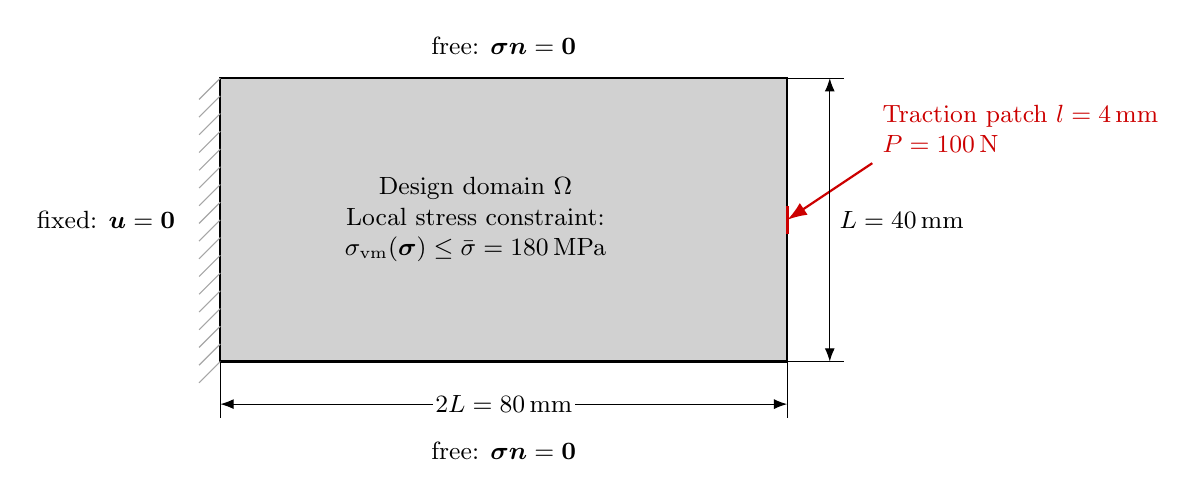
\begin{tikzpicture}[x=0.09cm,y=0.09cm,>=Latex]
  \def\L{80}
  \def\H{40}

  % ================= 设计域矩形 =================
  \draw[thick,fill=black!18] (0,0) rectangle (\L,\H);

  % ================= 左侧固支边界与阴影线 =================
  \draw[thick] (0,0) -- (0,\H);
  \foreach \y in {0,2.5,...,40} {
    \draw[gray!70] (0,\y) -- (-3,\y-3);
  }
  \node[font=\small,align=center,anchor=east] at (-5,0.5*\H)
    {fixed: $\boldsymbol{u}=\boldsymbol{0}$};

  % ================= 右侧中点载荷 (局部区间加载) =================
  \def\patchhalf{2} % 载荷宽度 4mm (y in 18..22)
  \draw[very thick,red!80!black] (\L,0.5*\H-\patchhalf) -- (\L,0.5*\H+\patchhalf);
  \draw[thick,-{Latex[length=2.5mm,width=1.8mm]},red!80!black] (\L+12,0.5*\H+8) -- (\L,0.5*\H)
    node[pos=0,above right,font=\small,align=left,red!80!black] {Traction patch $l=4\,\mathrm{mm}$\\$P = 100\,\mathrm{N}$};

  % ================= 尺寸标注 =================
  % 底部宽度标注
  \draw[thin] (0,0) -- (0,-8);
  \draw[thin] (\L,0) -- (\L,-8);
  \draw[<->,thin] (0,-6) -- (\L,-6)
    node[midway,fill=white,inner sep=1pt,font=\small] {$2L=80\,\mathrm{mm}$};

  % 顶部高度标注
  \draw[thin] (\L,0) -- (\L+8,0);
  \draw[thin] (\L,\H) -- (\L+8,\H);
  \draw[<->,thin] (\L+6,0) -- (\L+6,\H)
    node[midway,right,font=\small] {$L=40\,\mathrm{mm}$};

  % ================= 顶部与底部自由边界标注 =================
  \node[font=\small,align=center,anchor=south] at (0.5*\L,\H+2)
    {free: $\boldsymbol{\sigma}\boldsymbol{n}=\boldsymbol{0}$};
  \node[font=\small,align=center,anchor=north] at (0.5*\L,-10)
    {free: $\boldsymbol{\sigma}\boldsymbol{n}=\boldsymbol{0}$};

  % ================= 设计域内部说明 =================
  \node[font=\small,align=center] at (0.45*\L,0.5*\H)
    {Design domain $\Omega$\\Local stress constraint:\\$\sigma_{\mathrm{vm}}(\boldsymbol{\sigma}) \le \bar{\sigma} = 180\,\mathrm{MPa}$};

\end{tikzpicture}
\end{document}
